\quad{}
\item \textbf{{[}IJC/PRELIM/9597/2018/P2/Q5{]} }

The following security advisory was issued after the recent cyberattack
on SingHealth\textquoteright s IT system.
\begin{center}
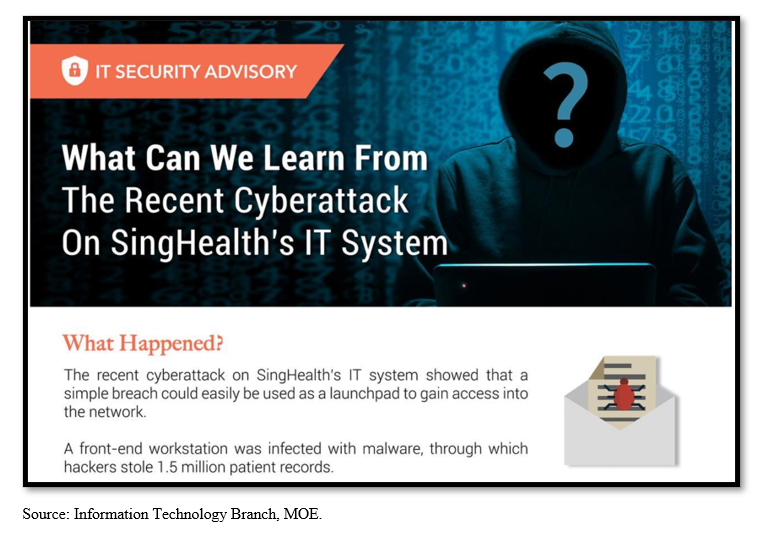
\includegraphics[width=0.5\paperwidth]{C:/Users/Admin/Desktop/Github/question_bank/LyX/static/img/9597-IJC-2018-P2-Q5-1}
\par\end{center}

Employees of SingHealth\textquoteright s group of hospitals are issued
with computing devices, which have access to patients\textquoteright{}
records stored on the SingHealth central server, via the internet.
Each employee is also issued with an email account for both internal
and external communications. 
\begin{enumerate}
\item Describe \textbf{two} differences between a client-server network
and a peer-to-peer network. \hfill{}{[}4{]}

\emph{\textquotedblleft \dots{} a simple breach could easily be used
as a launchpad to gain access into the network.\textquotedblright{}}
\item Describe how a breach could have happened and how patient records
were subsequently accessed. \hfill{}{[}4{]}
\begin{enumerate}
\item A further notice adds that \textquotedblleft \emph{Employees can practice
good personal data protection and cybersecurity habits in their place
of work.}\textquotedblright{}
\end{enumerate}
\item Describe \textbf{two} ways that this can be done. \hfill{} {[}2{]}
\item List \textbf{two} ways that SingHealth as an organisation can do to
ensure the security of their network. \hfill{}{[}2{]}
\end{enumerate}